\documentclass[11pt, a4paper]{article}

\usepackage[utf8]{inputenc}
\usepackage{graphicx}
\usepackage{color}
\graphicspath{{figures/pdf/}}

\title{Position Paper on  openETCS Development Work Flow and Associated Tools \\ The University of Bremen View}
\author{C\'ecile Braunstein \and Jan Peleska \and Johannes Feuser}
\date{\today}

\newcommand{\remark}[2] { \textcolor{red}{{\bf #1 :} #2}\par}
\newcommand{\todo}[1] { \textcolor{blue}{ #1\par}}
% Makes Marginpars easier to read
\setlength{\marginparwidth}{1.2in}
\let\oldmarginpar\marginpar
\renewcommand\marginpar[1]{\-\oldmarginpar[\raggedleft\footnotesize #1]%
{\raggedright\footnotesize #1}}

\newenvironment{inoutput}
{\vspace{2mm}
\noindent
\begin{tabular}{|r|p{.7\linewidth}|l|}
\hline}
{
\hline
\end{tabular}}

\begin{document}
\maketitle
\begin{abstract}
This document is a proposition from the openETCS team at University of Bremen about the 
work flow and resulting tool chain 
architecture definition as required for WP3a. The current contribution considers the ``left-hand side of the V-Model'', that is, the development-related flow and tools. We plan to investigate the V\&V-related
work flow and associated tools in the next sprint.
\end{abstract}


% -----------------------------------------------------------------------
\section{General work flow description -- Model-Driven Approach}
We advocate that  the tool chain should rely on the {\it model-driven} paradigm.
The use of domain-specific modelling concepts and an openETCS-specific domain framework is suitable for
formal verification and automated code generation, and presents high potential
for modelling railway control systems as advocated in 
\cite{RSRSChapter2012,DBLP:journals/fac/HaxthausenPK11,SecurityInOMS}.


% ..............................................................................
\paragraph{Model-driven work flow.}
The general notion of model-driven development considers software development as
a transformational approach where code is automatically derived from higher-level models.  
Figure~\ref{fig:model_hier} shows the typical model-driven process as characterised by the
Object Management Group \cite{OMGUML}. 
The \emph{Meta Metamodel} specifies the rules for defining new modelling formalisms.
It has to be sufficiently powerful to introduce language elements, syntactic and static semantic 
rules which are suitable for the domains -- in our case, the ETCS domain -- to be modelled. 

Using the rules of the meta metamodel, one or more domain-specific modelling formalisms are
specified by means of the \emph{metamodel}: the latter comprises all the language elements available and the rules to be observed when developing a concrete model in the specific formalism designed using the meta metamodel. In openETCS one might decide to introduce one or more formalisms for modelling the
EVC (European Vital Controller -- on board computer of ETCS trains) and track-side equipment (balises, track elements, interlocking systems, \ldots). It might even be useful to apply different formalisms for describing the EVC alone, since its functionality comprises many heterogeneous properties, such as odometric components and communication components, brake control and so on.

The availability of several formalisms has the advantage to allow for stronger specialisation per formalism, so that each of these uses a smaller amount of language
elements and fewer modelling rules. On the other hand it has the disadvantage that the semantics of interfaces between models elaborated with different formalisms has to be formally described.

A concrete \emph{Model} specifies functional and/or non-functional properties of the system (component) to be developed. A valid model has to observe the rules of the underlying metamodel. Syntactic and static-semantic conformance ensures that \emph{generators}  can produce \emph{high-level code} (C,C++, railway-specific programming languages, \ldots) from the model. 

This code is compiled and linked to the \emph{domain framework}, a collection of libraries or pre-defined services which are expected to be required by every (or at least most) applications in the domain.
In the openETCS context it has to be discussed, for example, whether it is desirable to specify a 
\emph{standardised operating system API} streamlined for ETCS, or, at least, for EVC applications: the applications to be modelled and generated will have to be embedded into a run-time environment executing the application code on the target HW platform. If the API of the run-time environment is not available in the domain framework, the API (and its associated behaviour) always has to be modelled in the
application models themselves, which would clutter the models in an unacceptable way.




% ...............................................................................
\paragraph{Availability of methods and tools.}
At each level of the hierarchy different
(open source and closed source) tools are already available, supporting  (at least partially) 
formal modelling semantics and formal model-to-model or
model-to-text transformations. The list we have provided is not exhaustive but we try
to enumerate the ones available and open.

For the meta metamodeling activity, we can choose among MOF \cite{MOF-spec},
Ecore \cite{EMF-Ecore} and GOPRR \cite{GOPRR}. 
The metamodel generation may then be done by the EMF eclipse plug-in \cite{Steinberg:2009:EEM:1197540}, and the 
concrete model may be obtained by a graphical and/or textual tool, here we can
also mention the powerful non-open tool MetaEdit+ \cite{MetaEdit} . 
Finally code may be generated (X-text/Xpand or OpenArchitectureWare part of the
Eclipse-EMF). University of Bremen can
also provide code generators, see section \ref{sec:codegeneration} for a brief
overview of our tool.



\begin{figure}[htbp]
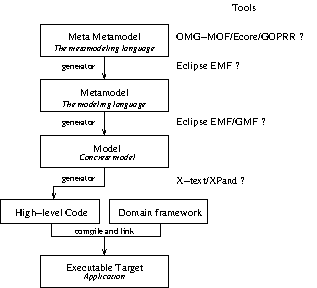
\includegraphics[width=\textwidth]{metamodelinghier.pdf}
\caption{The meta-modelling hierarchy}
\label{fig:model_hier}
\end{figure}
%\begin{itemize}
%\item Good way of modeling
%\item appropriate for ETCS
%\item so proof/formal model to mode / model to text
%\item some experiences cite paper ...
%\end{itemize}

% -----------------------------------------------------------------------
\section{How to choose ``good" (meta) meta-models}
We have  agreed that   WP2 should provide some requirements concerning the adequateness of modelling
languages. Nevertheless, in the context of model-driven
development,  one of the tasks of WP3a should be to determine what makes a good
candidate for meta-modelling from the tools perspective.
We think that we need to define criteria helping to discriminate between the
available modelling techniques and associated tools. 
The criterion should also refer to practical properties such as graphical/text
modelling, development costs, availability, open source etc. 

We also need to take into consideration the way the produced model will be used. 
Is our modelling language suitable for code generation in a simulation environment or  for a target platform, can we derive test cases and formal verification obligations from the model? 
The question boils down to: 
\begin{center}
Which features should the meta meta-model support ?
\end{center}

%\begin{itemize}
%\item Requirement from WP2 and maybe with a subset
%\item what do we need for to do with our model
%\item what are the criterion for a good metamodel
%\item Define criteria for the choice test cases, simulation, dev cost, open
%source
%\end{itemize}

% -----------------------------------------------------------------------
\section{The code generation}
\label{sec:codegeneration}
University of Bremen  already has some experiences with code generators. We can provide a
verified transformation from  model to intermediate model representation
(IMR) and the transformation from IMR to C/C++ code. Figure \ref{fig:generator}
shows the basic steps of our generator.  
\begin{figure}[htbp]
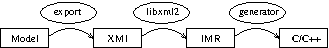
\includegraphics[width=\textwidth]{code_generator.pdf}
\caption{Uni Bremen Generators}
\label{fig:generator}
\end{figure}


Once we obtain the generated code, we need to investigate which Operating
system API standard  we should use. To ensure the soundness of our approach this
decision should be made early in the decision process. If the code generated
relies on the availability of specific operating system mechanism, we lost the
benefits of the model re-usability. According to our current state of information a candidate for 
and operating system has already been selected.



% -----------------------------------------------------------------------
\section{Certifiable open source -- HW standardisation versus virtualisation}
\label{sec:virtual}
A major difference between conventional open source projects and the openETCS approach is 
that the artefacts resulting from our work flow have to be certified. The availability of
(automatically) generated code is most beneficial if the associated V\&V artefacts can be used to obtain 
``immediate'' certification. Recalling that certification according to the
CENELEC standards EN50128, EN50129, EN50159 \cite{EN50129,EN50128,EN50159-1,
EN50159-2} requires V\&V of the binary
code, as integrated on the target hardware, we suggest to discuss two promising
options in the openETCS community:
\begin{itemize}
\item Operating system standardisation and HW standardisation: one computer architecture for all EVC developments 
\item Operating system standardisation and virtualisation: one virtual machine
running on different HW platforms providing their platform-specific hypervisor
\end{itemize}
Both options -- as explained below in more detail -- allow to provide open source
down to the binary code, both for  application and runtime environment. This would
allow to certify the binary code once-and-for-all, since it may run without
alterations in every target environment. Only changes in the application or in
the runtime environment would require re-certification.



The first option has been realised in the so-called  {\it Integrated Modular Avionics (IMA)} 
architecture. This approach reduces the development costs and
ensures safety and performances requirements by defining a platform with
a limited set of re-usable and interoperable hardware and software resources
Moreover, the interface between applications and the operating system has been standardised according to  the ARINC 653 standard  \cite{ARINC653P1-2}.



Another possibility is the use of hardware virtualisation. The advantage of this option is that
we may be able to handle different hardware suppliers and  different host operating
systems via the use of an hypervisor. The hypervisor makes it possible to run guest
operating systems simultaneously in virtual machine. It creates an abstraction
layer: the guest utilises a pre-defined hypervisor API  providing hardware
access \cite{tanenbaum2008}. 
The drawback is then to provide certified hypervisor. Nevertheless, the use of
hypervisor for safety-critical system has leaded to an important development of
safe-hypervisor over the last years
\cite{1629596,Garfinkel:2003:TVM:945445.945464,Wang:2010:HLA:1849417.1849986}. The openETCS project should benefit from
this active research area.


% =============================================================================
\section{Verification and Validation}


%The OpenETCS development process has to meet the standard CENELEC 50128
%\cite{EN50129,EN50128}. Some tools like the Eclipse plugin and toolkit TOPCASED
%\cite{TOPCASED} may be used to develop certified software.
%As far as we are aware of theses tools do not support the use of metamodel. 
%Shall we re-use such tool or do we have to provide new customized solition ?

\subsection{V\&V Options}
The verification and validation part will also  benefit from the  model
driven paradigm, both with respect to higher efficiency and quality.
\begin{itemize}
\item Test cases and test data and test procedures may be automatically derived from test models~\cite{PeleskaVL11Nfm,pel2011a}.

\item
Several alternatives exist for verifying code generated from models.
\begin{itemize}
\item The transformations used may be validated -- even formally verified -- once and for all, so that
the generation result is automatically regarded as correct.
\item The generation result may be automatically tested against its higher-level model: to this end, 
the model-based testing (MBT) approach can be used to create test suites conforming to the highest criticality level of the 
applicable CENELEC standards, in order to justify that the generated code is consistent to its model~\cite{PeleskaVL11Nfm,pel2011a,peleska2009d}.
\item The generated result may be formally verified against the model. (See~\cite{RSRSChapter2012,DBLP:journals/fac/HaxthausenPK11} for examples how to realise this.)
\end{itemize}
\end{itemize}


% ----------------------------------------------------------------------
\subsection{Activities and Tool Chain}\label{sec:activitychain}

Figure~\ref{fig:vandv} summarises the different engines we may need within
the development and V\&V process. 
% .....................................................................
\paragraph{Description of activities.}
A model-based approach to openETCS starts with the development of an openETCS 
model collection. This collection can be classified in several dimensions.
\begin{itemize}
\item Structuring according to EVC system components (odometry handler, communication handlers, management of state and level transitions etc.)
\item Structuring according to functional (input/output behaviour), structural (architecture)  and non-functional properties (for example, safety, security, reliability, availability  requirements)
\item Structuring according to different levels of abstraction (platform-independent model PIM, platform-specific model PSM)
\end{itemize}
The models are created within the syntactic and static semantic restrictions of the metamodel and
use   the informal Subset 026 of the ETCS specification as input.

Software development is based on the model collection. Though in principle, a fully automated model-based development approach could generate object code or even 
machine code directly from the models, we expect that it will be desirable to have high-level code (C, C++ or similar high-level languages) available since it is
easier to trace to the higher-level model than machine code. 

The right-hand side of Figure~\ref{fig:vandv} shows one part of V\&V activities. Their objective is to 
verify the consistency between models, high-level code and object/machine code.
\begin{itemize}
\item The openETCS model collection will be subject to the peer review of the openETCS community.

\item 
Additionally it is possible to perform complete property checking or incomplete simulations in order
to validate completeness and correctness of the models. For identification of properties the
conformance test cases specified in Subset~076 may be used, among other possibilities to specify validation properties.

\end{itemize}

On the left-hand side of the diagram further V\&V activities are listed.
For model-based system integration testing we propose to develop a second model, the {\it test model}
serving as the bases to model-based testing MBT; this is motivated below in Section~\ref{sec:mbti}.

As an alternative to property checking and simulation, test suites checking the consistency between
model (components) and generated object code can be generated from the input model, 
as described in Section~\ref{sec:comptest} below.




% .....................................................................
\paragraph{Manual versus automated activties.}
In principle, all activities identified in the rectangular boxes in Figure~\ref{fig:vandv} may be performed in a manual way. For the ideal approach, however, we recommend that 
\begin{itemize}
\item code generation,
\item compilation,
\item property checking, simulation  and testing,
\item model-based testing,
\item equivalence checking
\end{itemize}
are completely automated, 
so that only 
\begin{itemize}
\item openETCS model design,
\item model peer review,
\item test model design,
\item property identification 
\end{itemize}
remain manual activities.

In the following, we indicate the benefits of the
model-driven approach in the context of V\&V and focus on 
aspects where the team from University of Bremen may contribute.


% ---------------------------------------------------------------------
\subsection{Model-Based System Integration Testing}\label{sec:mbti}
The objectives of MBT on system integration level are to
\begin{itemize}
\item validate the correctness and completeness of the openETCS development model,
\item verify that the generated code components cooperate correctly on the target HW, in 
order to achieve the system-level 
capabilities.
\end{itemize}

The first objective implies that the {\it test model} and the original openETCS development model are
separate entities; otherwise the system integration test would just validate that all logical
errors still residing in the openETCS development model are really implemented in the code. Even in presence
of a formally validated development model, in which high confidence can be placed, we prefer to create a 
separate test model, because
\begin{itemize}
\item the test model may use a higher level of abstraction since only the SUT behaviour visible at the 
system interfaces is relevant,

\item the test model may specify different interfaces to the SUT, depending on the observable interfaces
in a test suite; the observation level ranges from black-box (only the ``real'' SUT system interfaces
are visible) to grey-box level (some global variables may be monitored or even manipulated by the testing environment, some task or object communications may be observed etc.),  

\item the development model may contain errors that are only revealed during HW/SW integration (for example, calculations failing due to inadequate register word size, or deadlines missed due to insufficient CPU resources).
\end{itemize}

We suggest to create test models on the basis of the ETCS standard (subset 026) and
the existing high-level test suites made available in subset 076. The latter test cases should 
be feasible computations of the test model, so that the test model really creates a {\it superset}
of the existing test suite from subset 076


% ---------------------------------------------------------------------
\subsection{Model-Based Component Testing}\label{sec:comptest}

The second application of MBT is for the objective of code verification.
If model-to-text and text-to-text transformations are not formally verified, it
is necessary to verify the outcome of each transformation. Since the transformation
source is a model $M$ (recall that also high-level code is regarded as a model, represented, for example, by its control flow graphs), MBT suites can be derived automatically from this model to show that the
generated code conforms to $M$. 

Observe that in contrast to system-level MBT no redundant model is used for this objective, but the
same model $M$ used for code generation can be used: we just have to verify the consistency between 
code and $M$, without validating $M$'s correctness and completeness. The latter task is separately performed
by means of 
\begin{itemize}
\item property checking or
\item simulation.
\end{itemize}


% ---------------------------------------------------------------------
\subsection{Property Checking}

Development models are checked with respect to internal consistency and completeness 
by means of model checkers capable of property checking. 


% ---------------------------------------------------------------------
\subsection{Availability of Tools}

A wide variety of model checking and MBT tools is available.
It has to be noted, however, that in a DSL approach we cannot expect that
these tools will be directly able to parse openETCS (sub-)models. Instead, these models
will have to be transformed into the formalisms understood by the tools.

\begin{itemize}
\item For MBT, the tool RT-Tester (see citations above) accepts different parser front ends 
to transform models into its own internal representation.
\item We plan to establish an openETCS-specifc open source variant based on RT-Tester during the openETCS project.

\item For model checkers several input languages are available. It still has to be investigated which tools are most appropriate, and then cross transformation for this tool has to be developed.
\end{itemize}




%
%% --------------------------------------------------------------
%%\subsection{From a metamodel to model}
%
%Figure~\ref{fig:vandv} summarises the different engines we may need within
%the development and V\&V process. In the following, we show the benefits of the
%model-driven approach in the context of V\&V and focus on 
%aspects where the team from University of Bremen may contribute.
%
%
%As explained in the previous section, we create a metamodel for a domain specific
%language from the ETCS standard. Using DSLs offers several advantages during the development and V\&V process. 
%First,  a DSL helps to map the natural language
%that describes the ETCS (Subset 026 \cite{subset026}) into a formal language. This favours a peer reviewing
%of the actual model against the original documents. Moreover, from the
%metamodel, one may derive ETCS standard models with formally defined syntax and
%static semantics. 
%The DSL may also be used to
%constrain hardware interfaces as defined in the documents, so that limited
%interfaces may be applied during modelling 
%
%Finally, it seems natural that the DSL should also be used to formalize the test
%plan \cite{subset076}. One advantage will be that this subset could also be
%checked for vacuity, consistency or coverage analysis. It can also be used to
%automatically derive properties or assertions for the source code. The formalized
%test plan may be re-used for dependability analysis and be applied early in the design process 
%at a high level of abstraction.
%
%The model should serve as a specification. It can be used to automatically
%generate property and test cases with or without the help of the formalized
%test plan. Uni. Bremen can provide techniques for automated model-based testing
%(see citations above). 
%
%% -----------------------------------------------------------------------------
%%\subsection{Source and object code verification}
%In \cite{RSRSChapter2012} a hazard analysis identifying the remaining safety and
%security threats still present when performing model-driven paradigm has been
%performed, and effective methods for countering each hazards have been proposed.
%
%In the paper, the authors advocate a model-to-text transformation to generate
%program source code  with a well defined semantics from the model. The
%program is simply lifted to the model and defined to be the model semantics,
%this facilitates the V\&V work flow considerably but implies validation obligation
%for the program source code.
%
%Validation of the source code should be made by combining techniques such as
%static program analysis by abstract interpretation, property checking,
%software testing.
%
%The remaining problem is to prove that the object code embedded into a target
%platform is really consistent with the program source.
%To check the compliance between source code and object code, we suggest an
%{\it object code verification} : each time an object code is generated, the
%generated object code is verified to be consistent with the source code. This
%method removes the constraint of having a verified compiler. It can be fully
%automated when the program code comes from a higher-level of abstraction, hence
%it is well-suited for a model-driven paradigm.
%
%
%The object code require certification when integrated to HW/SW platform, section
%\ref{sec:virtual} shows the benefits of hardware virtualisation
%
%\subsection{Best tools ?}
%Unlike the previous discussion about which tool is better suited for the
%openETCS platform, we think that the platform should be open to a big variety of
%verification and validation tools. 
%The openETCS should then provides a way to organized and classified the
%tools, for example with regards to the level of certification they may achieve.

\begin{figure} [htbp]
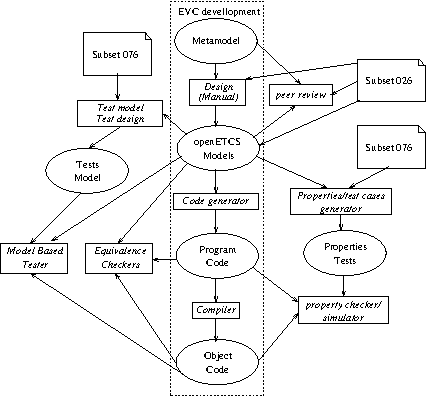
\includegraphics[width=\textwidth]{VandV.pdf}
\caption{Toolchain with V\&V. See Section~\ref{sec:activitychain} for explanations of activities and artefacts, as well as possible automation steps in a model-based approach.}
\label{fig:vandv}
\end{figure}
\bibliographystyle{alpha}
\bibliography{biblio} 
\end{document}
